\documentclass{book}

%%Packages:

\usepackage[utf8]{inputenc}
\usepackage[UKenglish]{babel}
\usepackage{graphicx}
\usepackage{cite}
\usepackage[hidelinks]{hyperref}
\usepackage{listings}
\usepackage{latexsym}
\usepackage{amsmath,amsthm,amssymb}
\usepackage{proof}
\usepackage{stmaryrd}
\usepackage{epstopdf}
\usepackage{pgf}
\usepackage{tikz}
\usepackage{algorithm}
\usepackage[noend]{algpseudocode}
\usetikzlibrary{automata,arrows,decorations.pathreplacing}
\usetikzlibrary{positioning}

%trick to avoid floating images trespassing sections boundaries
\usepackage[section]{placeins}

%margins
\usepackage{layout}
% \usepackage[inner=4cm,outer=2cm]{geometry}

%%Notation:

%%vectors
\renewcommand{\vec}[1]{\boldsymbol{#1}}
%%sets
\newcommand{\set}[1]{\mathcal{#1}}
%%matrixes
\newcommand{\mat}[1]{#1}
%%norm
\newcommand{\norm}[1]{\left\Vert #1 \right\Vert}
%%defeq
\newcommand{\defeq}{\triangleq}
%%
\newcommand{\net}[1]{\mathrm{#1}}


%%Envirorments:

% \newtheoremstyle{definition}{}{}{\itshape}{}{\bfseries}{.}{.5em}{\thmnote{#3's }#1}
\theoremstyle{definition}
\newtheorem{defn}{Definition}
\theoremstyle{definition}
\newtheorem{remark}{Remark}
\theoremstyle{definition}
\newtheorem{thm}{Theorem}

%Paths:

\graphicspath{ {./images/} }

\title{On recurrent neural networks}
\author{Giulio Galvan}

%%%%%%%%%%%%%%%%%%%%%%%%%%%%%%%%%%%%

\begin{document}
\maketitle
\tableofcontents
\chapter{Artificial neural networks}
  \section{A family of models}
  \input{chapter1/introduction_ann}
  \section{Feed forward neural networks}
  
A feed forward neural network is an artificial neural network in which there are no cycles, that is to say each layer output is \textit{fed} to the 
next one and connections to earlier layers are not possible. 


\begin{defn}[Feed forward neural network]
\label{def_ffnn}
A feed forward neural network is tuple:
$$\net{FFNN}\defeq \langle\vec{p},\set{W},\set{B},\sigma(\cdot),F(\cdot)\rangle$$
\begin{itemize}
 \item $\vec{p} \in \mathbb{N}^U$ is the vector whose elements $p(k)$ are the number of neurons of layer $k$; $U$ is the number of layers
 \item $\set{W} \defeq \{W^k_{p(k+1) \times p(k)}, k=1,...,U-1 \}$ is the set of weight matrices of each layer
 \item $\set{B} \defeq \{\vec{b}^k \in \mathbb{R}^{p(k)}, k=1,...,U \} $ is the set of bias vectors
 \item $\sigma(\cdot): \mathbb{R}\rightarrow \mathbb{R}$ is the activation function
 \item $F(\cdot): \mathbb{R}^{p(U)}\rightarrow \mathbb{R}^{p(U)}$ is the output function.
\end{itemize}
\end{defn}

\begin{remark}{}
Given a $\net{FFNN}$:
\begin{itemize}
 \item The number of output units is $p(U)$
 \item The number of input units is $p(1)$
 \item The total number of weights is $\mathcal{N}(\set{W}) \defeq \sum_{k=1}^{U-1} p(k+1)p(k)$
 \item The total number of biases is $\mathcal{N}(\set{B}) \defeq \sum_{k=2}^{U} p(k)$.
\end{itemize}
\end{remark}

\begin{defn}[Output of a $\net{FFNN}$]
Given a $\net{FFNN}$ and an input vector $\vec{x} \in \mathbb{R}^{p(1)}$ the output of the net $\vec{y} \in \mathbb{R}^{p(U)}$  is defined by the following:

\begin{align}
&\vec{y}=F(\vec{a}^{U}) &\\
&\vec{h}^{i} \defeq \sigma(\vec{a}^{i}), & i=2,...,U\\
&\vec{a}^{i} \defeq W^{i-1} \cdot \vec{h}^{i-1} +\vec{b}^i  & i=2,...,U\\
&\vec{h}^{1} \defeq \vec{x}.u &
\end{align}
\end{defn}

\subsection{Learning with FFNNs}
A widespread application of neural networks is that of machine learning. In the following we will model an optimization problem which rely on $\net{FFNNs}$.
To model an optimization problem we first need to define a dataset $D$ as 
\begin{equation}
D\defeq\{\overline{\vec{x}}^{(i)} \in \mathbb{R}^p, \overline{\vec{y}}^{(i)} \in \mathbb{R}^q,  i=1,...,N\}
\end{equation}
The dataset $D$ is composed of $N$ training examples $\overline{\vec{x}}^{(i)}$, each one of them paired with a label $\overline{\vec{y}}^{(i)}$.

Then we need a loss function $L_D:\mathbb{R}^{\mathcal{N}(\set{W})+\mathcal{N}(\set{B})} \rightarrow \mathbb{R}_{\geq 0}$ over $D$ defined as
\begin{equation}
L_D(\set{W},\set{B})\defeq\frac{1}{N}\sum_{i=1}^N L(\overline{\vec{y}}^{(i)},\vec{y}^{(i)}(\set{W},\set{B})) 
\end{equation}
$L(\overline{\vec{y}},\vec{y}):\mathbb{R}^{p(U)} \times \mathbb{R}^{p(U)} \rightarrow \mathbb{R}$ is an arbitrary loss function computed on the $i^{th}$ example. Note that $\vec{y}$ is the output of the
network, so it depends on $\set{W}$ and $\set{B}$ whether $\overline{\vec{y}}$ is fixed within the dataset.


The problem is then to find a $\net{FFNN}$ which minimize $L_D$. As we have seen feed forward neural networks allow for large customization: the only variables in the optimization problem are the weights
and the biases, the other
parameters are called \textit{hyper-parameters} and are determined \textit{a priori}. Usually the output function is chosen depending on what we are trying to learn, for instance for k-way classification
is generally used the \textit{softmax} function \begin{equation}
softmax(x)_i\defeq \frac{e^{\vec{x}_i}}{\sum_{j=1}^k e^{\vec{x}_j} },
\end{equation} for regression a simple identity function.
For what concerns the number of layers and the number of units per layers they are chosen relying on experience or performing some kind of hyper-parameter tuning, which usually consists on training nets
with some different configurations of such parameters and choosing the 'best one'.

Once we have selected the values for all hyper-parameters the optimization problem becomes:

\begin{equation}
\min_{\set{W},\set{B}} L_D(\set{W},\set{B}) \\
\end{equation}


\subsection{Gradient}
\subsection{Gradient}

We can compute partial derivatives with respect to a single weight $w_{lj}$, using simply the chain rule, as 

$$\frac{\partial L}{\partial w_{lj}}=\frac{\partial L}{\partial a_l} \cdot \frac{\partial a_l}{\partial w_{lj}}=\delta_l \cdot \phi_j$$
where we put

\begin{equation}
\delta_l \triangleq \frac{\partial L}{\partial a_l}
\end{equation}



So we can easily compute $\delta_u = \frac{\partial L^{(i)}}{\partial a_u} $ for each output unit $u$ once we choose a differentiable loss function; note
that we don't need the weights for such a computation. 

Let $P(l)$ be the set of parents of neuron $l$, formally:
\begin{equation} 
P(l) = \{ k: \exists \text{ a link between $l$ and $k$ with weight } w_{lk} \}
\end{equation}

Again, simply using the chain rule, we can write, for each non output unit $l$:

\begin{equation}
\label{loss_deriv}
\delta_l = \sum_{k\in P(l)} \frac{\partial L^{(i)}}{\partial a_k} \cdot \frac{\partial a_k}{\partial a_l}= \sum_{k\in P(l)} \delta_k \cdot 
\frac{\partial a_k}{\partial \phi_l} \cdot \frac{\partial \phi_l}{\partial a_l} = \sum_{k\in P(l)} \delta_k \cdot 
w_{kl} \cdot \sigma'(a_l)
\end{equation}


For output units instead we can compute $\delta_u = \frac{\partial L^{(i)}}{\partial a_u} $ directly once we define the loss function.

For biases variables partial derivatives are simply given by:
$$\frac{\partial L}{\partial b_{l}}=\frac{\partial L}{\partial a_l} \cdot \frac{\partial a_l}{\partial w_{l}}=\delta_l \cdot 1$$




In the following we rewrite the previously derived equations in matrix notation.
Let us recall that the weight matrix for the $i^{th}$ layer is the $p(i) \times p(i-1)$ matrix whose elements $w_{l,k}$ are the weights of the arcs which link neuron $k$ from level $i-1$ to neuron $l$ from level $i$, where
$p(i)$ is the number of neuron layer $i$ is composed of.


We can rewrite equation \ref{loss_deriv} in matrix notation as:

\begin{equation}
 \frac{\partial L}{\partial W^i} = \frac{\partial L}{\partial \vec{a}^{i}} \cdot\Big(\frac{\partial \vec{a}^{i}}{\partial W^i}\Big)^T =
 \Delta^i \cdot (\vec{\phi}^{i-1})^T
\end{equation}

where
\begin{equation}
\Delta^i  \triangleq  \frac{\partial L}{\partial \vec{a}^{i}} 
\end{equation}

\begin{equation}
 \Delta^i = \big(W^{i+1}\big)^T \cdot \Delta^{i+1} \circ \sigma(\Delta^i)
\end{equation} 

\begin{equation}
 \frac{\partial L}{\partial b^i} = \frac{\partial L}{\partial \vec{a}^{i}} \cdot\Big(\frac{\partial \vec{a}^{i}}{\partial b^i}\Big)^T =
 \Delta^i \cdot Id
\end{equation} 



  \section{Recurrent neural networks}
  Recurrent neural networks differ from feed foward neural networks because of the presence of recurrent connections: at least one perceptron output at a given layer $i$ is \textit{fed} to another perceptron
at a level $j<i$, as can be seen in figure \ref{rnn_model}. This is a key difference: as we will see in the next section, rnn are not only more powerfull than ffnn but as powerfull as turing machines.


\tikzstyle{rnn_style}=[->,shorten >=1pt,auto,node distance=1.5cm,
  thick,
  neuron/.style={circle,fill=white!50,node distance =1.2cm,draw,minimum size=0.7cm,font=\sffamily\Large\bfseries},
  missing/.style={rectangle,node distance =1.2cm,fill=white!50,draw=none,minimum size=0.7cm,font=\sffamily\Huge\bfseries},
  label/.style={node distance=1.2cm,rectangle,fill=white!50,draw=none,minimum size=0.7cm,font=\sffamily\normalsize},
  layer/.style={rectangle,fill=white!50,draw,minimum width=4cm,font=\sffamily\normalsize},
  loopStyle/.style={in=120,out=60, distance=2.5cm},]
\begin{figure}[h!]
 \centering
\begin{tikzpicture}[rnn_style]

  \node[neuron]    (x0)       {};
  \node[neuron]    (x1)[right of=x0]   {};
  \node[neuron]    (x2)[right of=x1]   {};
  \node[missing]   (x3)[right of=x2]   { $\hdots$};
  \node[neuron]    (xn)[right of=x3]   {};
  
  \node[label]    (u0)[below of=x0]   {$u_0[t]$};
  \node[label]    (u1)[below of=x1]   {$u_1[t]$};
  \node[label]    (u2)[below of=x2]   {$u_2[t]$};
  \node[label]    (un)[below of=xn]   {$u_n[t]$};
  
  
  
  \node[layer] (hl)[above of=x2,node distance=2cm] {Hidden layer};
  \node[neuron](b) [right of=hl,node distance=3cm] {};
  \node[label] (b_l) [right of=b] {bias=1};
  \node[layer] (ol)[above of=hl,node distance=2cm] {Output layer};
  
  \node[neuron] (o1) at (0,5.5) {};
  \node[neuron] (o2)[right of=o1] {};
  \node[neuron] (o3)[right of=o2] {};
  \node[missing](o4)[right of=o3] {$\hdots$};
  \node[neuron] (on)[right of=o4] {};
  
  
  \node[label]    (y0)[above of=o1]   {$y_0[t]$};
  \node[label]    (y1)[above of=o2]   {$y_1[t]$};
  \node[label]    (y2)[above of=o3]   {$y_2[t]$};
  \node[label]    (yn)[above of=on]   {$y_n[t]$};
  
  
  \path[->] (x0) edge [] node[]{$W_{in}$}   (hl)
	    (x1) edge []   (hl)
	    (x2) edge []   (hl)
	    (xn) edge []   (hl)
	    (u0) edge []   (x0)
	    (u1) edge []   (x1)
	    (u2) edge []   (x2)
	    (un) edge []   (xn)
	    (ol) edge []   (o1)
	    (ol) edge []   (o2)
	    (ol) edge []   (o3)
	    (ol) edge []   (on)
	    (o1) edge []   (y0)
	    (o2) edge []   (y1)
	    (o3) edge []   (y2)
	    (on) edge []   (yn)
	    (hl) edge []  node[]{$W_{out}$} (ol)
	    (b)  edge [bend left,dotted,in= 160]  node[]{$b_{rec}$} (hl)
	    (b)  edge [bend left,dotted,anchor=west, in= -160]  node[]{$b_{out}$} (ol)
	    (hl) edge [loop ,in=-160,out=160, distance=3cm,anchor=east ]      node [align=center]  {$W_{rec} $} (hl);


\end{tikzpicture}
\caption{Rnn model}
\label{rnn_model}
\end{figure}



This difference in topology reflects also on the network's input and output domain, where in feed foward neural networks inputs and outputs were real valued vectors, recursive neural networks deal with
sequences of vectors, that is to say that now time is also considered. One may argue that taking time (and sequences) into consideration is some sort of limitation because it restricts our model to deal only
with a temporal inputs; that's not true, in fact we can apply rnn to non temporal data by considering space as the temporal dimension or we can feed the network with the same input for all time steps, or just
providing no input after the first time step.

\begin{defn}[Recurrent neural network]
\label{def_rnn}
A recurrent  neural network is tuple
$$RNN\triangleq< \set{W},\set{B} ,\sigma(\cdot),F(\cdot)>$$
\begin{itemize}
 \item $\set{W} \triangleq \{\mat{W}^{in},\mat{W^{rec},\mat{W^{out}}}\}$ where
 \begin{itemize}
  \item $W^{in}$ is the $r\times p$ input weight matrix
  \item $W^{rec}$ is the $r\times r$ recurrent weight matrix
  \item $W^{out}$ is the $o \times r$ output weight matrix
 \end{itemize}
 \item $\set{B} \triangleq \{\vec{b^{rec},\vec{b^{out}}}\}$ where
 \begin{itemize}
   \item $\vec{b}^{rec} \in \mathbb{R}^{r}$ is the bias vector for the recurrent layer
   \item $\vec{b}^{out} \in \mathbb{R}^{o}$ is the bias vector for the output layer
 \end{itemize}
 \item $\sigma(\cdot): \mathbb{R}\rightarrow \mathbb{R}$ is the activation function
 \item $F(\cdot): \mathbb{R}^{o}\rightarrow \mathbb{R}^{o}$ is the output function
\end{itemize}
\end{defn}

\begin{remark}{}
Given a RNN
\begin{itemize}
 \item The total number of weights si given by $\mathcal{N}(W) \triangleq rp+r^2+ro$
 \item The number of biases by $\mathcal{N}(b) \triangleq r+o $
 \item $p$ is the size of input vectors, 
 \item$r$ is the number of hidden units
 \item $o$ is the size of output vectors. 
\end{itemize}
\end{remark}

\begin{defn}[Output of a RNN]
Given a $RNN$ and an input sequences $\{\vec{x}\}_{t=1,...,T}, \vec{x}_t \in \mathbb{R}^p$ the output sequence $\{\vec{y}\}_{t=1,...,T}, \vec{y}_t \in \mathbb{R}^o$ of the net is defined by the following:
\begin{align}
&\vec{y}_t \triangleq F(W^{out}\cdot\vec{a}_t + \vec{b}^{out})\\
&\vec{a}_t \triangleq W^{rec}\cdot\vec{\phi}_{t-1}+W^{in}\cdot\vec{x}_t+\vec{b}^{rec}\\
&\vec{\phi}_t \triangleq  \sigma(\vec{a}_t)
\end{align}
\end{defn}


As we can understand from definition \ref{def_rnn}, there is only one recurrent layer, whose weights are the same for each time step, so one can asks where does the deepness of the network come from.
The answer lies in the temporal unfolding of the network, in fact if we unfold the network step by step we obtain a structure similar to the structure of a feed foward neural network. As we can observe
in figure \ref{rnn_unfolding}, the unfolding of the network through time consist of putting identical version of the same reccurent layer on top of each other and linking the inputs of one layer to the
next one. The key difference from feed foward neural networks if, as we have already observed, that the weights in each layer are identical, and of course the additional timed inputs which are different for
each unfolded layer.

\tikzstyle{rnn_style}=[->,shorten >=1pt,auto,node distance=1.5cm,
  thick,
  neuron/.style={circle,fill=white!50,draw,minimum size=0.7cm,font=\sffamily\Large\bfseries},
  missing/.style={circle,fill=white!50,draw=none,minimum size=0.7cm,font=\sffamily\Huge\bfseries},
  label/.style={node distance=1.2cm,rectangle,fill=white!50,draw=none,minimum size=0.7cm,font=\sffamily\normalsize},
  layer/.style={rectangle,fill=white!50,draw,minimum width=4cm,font=\sffamily\normalsize},
  loopStyle/.style={in=120,out=60, distance=2.5cm},]
\begin{figure}[h!]
 \centering
\begin{tikzpicture}[rnn_style]

  %t=0
  \node[layer] (hl1) {Hidden layer t=0};
  
  \node[neuron]    (x0)[below left=0.3cm and 1cm of hl1]       {};
  \node[label]    (u0)[left of=x0]   {$\vec{x}_1$};
  

  
  \node[neuron] (o0) [above right=0.3cm and 1cm of hl1] {};
  \node[label]    (y0)[right of=o0]   {$\vec{y}_1$};
  
  %t=1
  \node[layer] (hl2)[above of=hl1,node distance=2.5cm] {Hidden layer t=1};
  
  \node[neuron]    (x1)[below left=0.3cm and 1cm of hl2]      {};
  \node[label]    (u1)[left of=x1]   {$\vec{x}_2$};
  
    
  \node[neuron] (o1) [above right=0.3cm and 1cm of hl2] {};
  \node[label]    (y1)[right of=o1]   {$\vec{y}_2$};
  
  %dots
  \node[label,font=\sffamily\Huge\bfseries] (hld)[above of=hl2,node distance=2cm] {$\hdots$};
  
  %t=T
  \node[layer] (hlT)[above of=hld,node distance=2cm] {Hidden layer t=T};
  
  \node[neuron]    (xT)[below left=0.3cm and 1cm of hlT]      {};
  \node[label]    (uT)[left of=xT]   {$\vec{x}_T$};
  
    
  \node[neuron] (oT) [above right=0.3cm and 1cm of  hlT] {};
  \node[label]    (yT)[right of=oT]   {$\vec{y}_T$};
  
  
  %biases
  \node[neuron](b) [right of=y1,node distance=2cm] {};
  \node[label] (b_l) [right of=b] {bias=1};

  
  \path[->] (x0) edge [bend right] node[]{$W^{in}$}   (hl1)
	    (u0) edge []   (x0)
	    (o0) edge []   (y0)
	    (x1) edge [bend right] node[]{$W^{in}$} (hl2)
	    (u1) edge []   (x1)
    	    (o1) edge []   (y1)
	    (xT) edge [bend right] node[]{$W^{in}$} (hlT)
	    (uT) edge []   (xT)
    	    (oT) edge []   (yT)

	    
	    (hl1) edge [bend left]  node[]{$W^{out}$} (o0)
    	    (hl2) edge [bend left]  node[]{$W^{out}$} (o1)
    	    (hlT) edge [bend left]  node[]{$W^{out}$} (oT)

	    (b)  edge [bend left,dotted,in = 90]  node[]{$b^{out}$} (o0)
	    (b)  edge [bend left, dotted, in = 90,out=80]  node[]{$b^{rec}$} (hl1)
	    (b)  edge [bend left, dotted]  node[]{$b^{rec}$} (hl2)
	    (b)  edge [bend left,dotted]  node[]{$b^{out}$} (o1)
	    (b)  edge [bend left, dotted,in = 200]  node[]{$b^{rec}$} (hlT)
	    (b)  edge [bend left,dotted,in =200]  node[]{$b^{out}$} (oT)
	    (hl1) edge [] node[]{$W^{rec} $} (hl2)
       	    (hl2) edge [] node[]{$W^{rec} $} (hld)
    	    (hld) edge [] node[]{$W^{rec} $} (hlT);



\end{tikzpicture}
\caption{Unfolding of a rnn}
\label{rnn_unfolding}
\end{figure}


\subsection{Learning with ffnn}
We can model an optimization problem in the same way we did for feed foward neural networks, the main difference is, again, that we now deal with temporal sequences so we need a slightly different
loss function.
Given a dataset $D$:
\begin{equation}
D\triangleq\{\{\overline{\vec{x}}\}_{t=1,...,T}, \overline{\vec{x}}_t \in \mathbb{R}^p, \{\overline{\vec{y}}\}_{t=1,...,T}, \overline{\vec{y}}_t \in \mathbb{R}^o;  i=1,...,N\}
\end{equation}
we define a loss function $L_D:\mathbb{R}^{\mathcal{N}(W)+\mathcal{N}(b)} \rightarrow \mathbb{R}_{\geq 0}$ over $D$  as
\begin{equation}
L_D(\set{W},\set{B})\triangleq\frac{1}{N}\sum_{i=1}^N \sum_{t=1}^T L_t(\overline{\vec{x}}_t^{(i)},\vec{y}_t^{(i)}) 
\end{equation}
$L_t$ is an arbitrary loss function at time step $t$.

The definition takes into account the output for each temporal step, depending on the task at hand, it could be relevant or not to consider intermediate
outputs; that's not a limitation, in fact we could define a loss which is computed only on the last output vector, at time $T$, and adds 0 for each
other time step.


\subsection{Gradient}
Consider a $\net{RNN}=\langle\set{W},\set{B},\sigma(\cdot),F(\cdot)\rangle$. Let $L_t:\mathbb{R}^o \times \mathbb{R}^o \rightarrow \mathbb{R}$ a loss function and  $g_t(\cdot):\mathbb{R}^{\mathcal{N}(\set{W})+\mathcal{N}(\set{B})} \rightarrow \mathbb{R}$ be the function defined by
$$g_t(\set{W},\set{B}) \triangleq L_t(F(\vec{y}^t(\set{W},\set{B})))$$
and $$g(\set{W},\set{B}) \triangleq \sum_{t=1}^T g_t(\set{W},\set{B})$$


\begin{align}
\frac{\partial g}{\partial \mat{W}^{rec}} &= \sum_{t=1}^T \nabla L_t^T \cdot J(F) \cdot \frac{\partial \vec{y}^t}{\partial \vec{a}^t} \cdot \frac{\partial \vec{a}^t}{\partial \mat{W}^{rec}}\\
&= \sum_{t=1}^T\frac{\partial g_t}{\partial \vec{a}^t} \cdot \frac{\partial \vec{a}^t}{\partial \mat{W^{rec}}}
\end{align}

As we noticed for $\net{FNNs}$ it's easy to compute $\frac{\partial g_t}{\partial \vec{a}^t}$ once we define $F(\cdot)$ and $L(\cdot)$, note that the weights are not involved in such computation.
Let's see how to compute $\frac{\partial \vec{a}^t}{\partial \mat{W}^{rec}}$.

Let's consider a single output unit $u$, and a weight $w_{lj}$, we have

\begin{align}
 \label{sum_over_time}
 \frac{\partial a^t_u}{\partial w_{lj}} &= \sum_{k=1}^t \frac{\partial a_u^t}{\partial a^k_l} \cdot \frac{\partial a^k_l}{\partial w_{lj}}\\
 &= \sum_{k=1}^t \delta^{tk}_{lu} \cdot \phi_j^{t-1}
\end{align}
where
\begin{equation}
\delta_{lu}^{tk} \triangleq \frac{\partial a_u^t}{\partial a^k_l}.
\end{equation}

Let's observe a first difference from FFNN case: since the weights are shared in each unfolded layer, in equation \ref{sum_over_time} we have to sum over time.

Let $P(l)$ be the set of parents of neuron $l$, defined as the set of parents in the unfolded network.

\begin{equation}
 \delta_{lu}^{tk} = \sum_{h\in P(l)} \delta_{hu}^{tk} \cdot \sigma'(a_h^{t-1})\cdot w_{hl}
\end{equation}

In Figure \ref{deriv_arcs_rnn} we can see the arcs which are involved in the derivatives in the unfolded network.

\tikzstyle{rnn_style}=[->,shorten >=1pt,auto,node distance=1.5cm,
  thick,
  neuron/.style={circle,fill=white!50,draw,minimum size=0.7cm,font=\sffamily\normalsize},
  missing/.style={circle,fill=white!50,draw=none,minimum size=0.7cm,font=\sffamily\Huge\bfseries},
  label/.style={node distance=1.2cm,rectangle,fill=white!50,draw=none,minimum size=0.7cm,font=\sffamily\normalsize},
  thick_edge/.style={line width=1.2pt},
  thin_edge/.style={line width=0.5pt}
  ]
\begin{figure}
 \centering
\begin{tikzpicture}[rnn_style]

  
  \node[neuron]    (x1)[]   {$u$};
  \node[neuron]    (x2)[right of=x1]   {$l$};
  \node[neuron]    (x3)[right of=x2]   {};
  \node[label]     (xl)[left of=x1] {$t$};
  
  \node[neuron]    (h1)[below of =x1]   {$u$};
  \node[neuron]    (h2)[right of=h1]   {$l$};
  \node[neuron]    (h3)[right of=h2]   {};
  \node[label]     (hl)[left of=h1] {$\hdots$};
  
  \node[neuron]    (y1)[below of=h1]   {$u$};
  \node[neuron]    (y2)[right of=y1]   {$l$};
  \node[neuron]    (y3)[right of=y2]   {};
  \node[label]     (yl)[left of=y1] {$k+2$};

  
  \node[neuron]    (z1)[below of=y1]   {$u$};
  \node[neuron]    (z2)[right of=z1]   {$l$};
  \node[neuron]    (z3)[right of=z2]   {};
  \node[label]     (zl)[left of=z1] {$k+1$};
  
  \node[neuron]    (w1)[below of=z1]   {$u$};
  \node[neuron]    (w2)[right of=w1]   {$l$};
  \node[neuron]    (w3)[right of=w2]   {};
  \node[label]     (wl)[left of=w1] {$k$};

  
%   \node[label]      (lu)[left of=u] {$u$};
%   \node[label]      (ll)[left of=z1] {$l$};


  \path[->] (h1) edge [thick_edge]  (x1)
	    (h1) edge [thin_edge]   (x2)
	    (h1) edge [thin_edge]   (x3)
	    (h2) edge [thick_edge]  (x1)
	    (h2) edge [thin_edge]   (x2)
	    (h2) edge [thin_edge]   (x3)
	    (h3) edge [thick_edge]  (x1)
	    (h3) edge [thin_edge]   (x2)
	    (h3) edge [thin_edge]   (x3);

  \path[->] (y1) edge [thick_edge]   (h1)
	    (y1) edge [thick_edge]   (h2)
	    (y1) edge [thick_edge]   (h3)
	    (y2) edge [thick_edge]   (h1)
	    (y2) edge [thick_edge]   (h2)
	    (y2) edge [thick_edge]   (h3)
	    (y3) edge [thick_edge]   (h1)
	    (y3) edge [thick_edge]   (h2)
	    (y3) edge [thick_edge]   (h3);
  
  
  \path[->] (z1) edge [thin_edge]   (y1)
	    (z1) edge [thick_edge]  (y2)
	    (z1) edge [thin_edge]   (y3)
	    (z2) edge [thick_edge]  (y1)
	    (z2) edge [thick_edge]  (y2)
	    (z2) edge [thick_edge]  (y3)
	    (z3) edge [thin_edge]   (y1)
	    (z3) edge [thin_edge]   (y2)
	    (z3) edge [thin_edge]   (y3);
	    
  \path[->] (w1) edge [thin_edge]   (z1)
	    (w1) edge [thick_edge]  (z2)
	    (w1) edge [thin_edge]   (z3)
	    (w2) edge [thin_edge]   (z1)
	    (w2) edge [thin_edge]   (z2)
	    (w2) edge [thin_edge]   (z3)
	    (w3) edge [thin_edge]   (z1)
	    (w3) edge [thin_edge]   (z2)
	    (w3) edge [thin_edge]   (z3);

	    


\end{tikzpicture}
\caption{Nodes involved in $\frac{\partial a^t_u }{\partial a^k_l}$.}
\label{deriv_arcs_rnn}
\end{figure}

In matrix notation we have:

\begin{equation}
 \frac{\partial \vec{a}^t}{\partial \mat{W}^{rec}} = \sum_{k=1}^t \frac{\partial \vec{a}^t}{\partial \vec{a}^k} \cdot \frac{\partial^+ \vec{a}^k}{\partial \mat{W}^{rec}}
\end{equation}


\begin{equation}
\frac{\partial^+ a^{k}}{\partial \mat{W}_j^{rec}} =
 \begin{bmatrix}
   \phi_j^{k}    & 0                & \cdots      & \cdots       & 0  \\
   0               & \phi_j^{k}     & \cdots      & \cdots       & 0  \\
   \vdots          & \vdots           & \ddots      & \vdots       &\vdots\\
   0               & \cdots           & \cdots      & \cdots       & \phi^{k}_{j}
\end{bmatrix}
\end{equation}

\begin{equation}
\triangleq \mat{\Delta}^{tk}
\end{equation}

\begin{align}
\mat{\Delta}^{tk} &= \mat{\Delta}^{t(k+1)} \cdot diag(\sigma'(\vec{a}^k)) \cdot \mat{W}^{rec} \\
&= \prod_{i=t-1}^{k} diag(\sigma'(\vec{a}^i)) \cdot \mat{W}^{rec}
\label{rnn_delta}.
\end{align}

The derivatives with respect to $\mat{W}^{in}$ and $\vec{b}^{rec}$ have the same structure.
The derivatives with respect to $W^{out}, b^{out}$ are straightforward:

\begin{equation}
\frac{\partial \vec{g}}{\partial \mat{W}^{out}} = \sum_{t=1}^T \frac{\partial g_t}{\partial \vec{y}^t} \cdot J(F) \cdot \frac{\partial \vec{y}^t}{\partial \mat{W}^{out}}
\end{equation}

\begin{equation}
\frac{\partial \vec{g}}{\partial \vec{b}^{out}} = \sum_{t=1}^T \frac{\partial g_t}{\partial \vec{y}^t} \cdot J(F) \cdot \frac{\partial \vec{y}^t}{\partial \vec{b}^{out}}.
\end{equation}

\paragraph{Back-propagation through time (BPTT)}
\textit{Back-propagation through time} is an extension of the \textit{back-propagation} algorithm we described for FNNs, we can think of BPTT
simply as a standard BP in the unfolded network. The same considerations done for BP also apply for BPTT, the difference is of course in how derivatives
are computed, equation \ref{rnn_delta}. Time complexity is easily derived noticing that in the unfolded network there are $n \cdot T$ units, where $n$ is the number of units of the RNN .This
yields time complexity $\mathcal{O}(\mathcal{N}(\set{W})\cdot T)$. Please see \cite{Williams90anefficient} for more details.








\subsection{The vanishing and exploding gradient problem}
The training of recurrent neural networks is afflicted by the so called \textit{exploding} and \textit{vanishing} gradient problem.
Such problem is directly linked to the notion of memory. When we talk about memory what are we really talking about is the dependecy of neuron output at a given time $t$ from previous time steps,
that is how $\phi^t$ depends on $\phi^{k}$ with $t>k$. This dependecy is captured by the expression $\frac{\partial \vec{a}^t}{\partial \vec{a}^k}$.
Obiuvsly when such expression equals zero it means neuron output at time $t$ is not affected by output at time $k$.
The terms $\frac{\partial \vec{a}^t}{\partial \vec{a}^k}$ are usually referred as \textit{long term} contribution when $k<<t$ or \textit{short term} contributions
otherwise.
We talk of \textit{exploding} gradient problem when \textit{long term} components grow exponentially, on the contrary of \textit{short term} ones, causing
the overall norm of the gradient to explode.
We refer to \textit{vanishing} gradient problem when, vice versa, \textit{long terms} diminish exponentially.

\textit{Vanishing} gradient means long term components approach zero value, this in turn leads to the fact that the output of the net won't depend on inputs of distant temporal steps, i.e the output
sequence is determined only using recent temporal input: we say that the network doesn't have memory. Evidently this can have catastrofic effects on the classification error. Imagine we would like
to classiy an input sequence as positive wheter or not it contains a zero character. It would seem a rather easy task, a task other classification models wouldn't have difficulties with. If the neural network
we are trainign has \textit{vanishing} gradient issue, it means it perform classification only using the most recent temporal input. What if the zero character was at the beginning of the sequence? Of course
the predicition would be wrong.

\textit{Exploding} gradient seems to be a different kind of a problem, it does not affect the ability of the network to use information from distant temporal step, on the contrary we have very strong
information about where to go. One could argue that some components, namely, the long term ones, have gradient norm exponentially bigger than short term ones. I fail to see why this could be a problem:
of course output of the first time stepes influences all successive steps, so changing the output of a long term neuron do imply big changes in the output of more distant in time neurons.
The only reason i see for considering this a problem is that big gradient norm, in general, is a problem if we are using algortithms like gradient descent with constant step.
If we are to compute a step in the gradient direction with a fixed step and gradient has too big norm we may make a too big step.

Let's now return to the nature of the problem and try to explaining the mechanics of it.

We have seen in the previous section that
\begin{equation}
\frac{\partial \vec{a}^t}{\partial \vec{a}^k} = \prod_{i=t-1}^{k}  diag(\sigma'(\vec{a}^i)) \cdot \mat{W}^{rec}
\label{memory_eq}
\end{equation}
Intuitively we can understand why such problems arises, more evidently in \textit{long term} components, just by looking at equation \ref{memory_eq};
We can notice each temporal contribution is the product of $l=t-k-1$ jacobian matrix, so in \textit{long term} components $l$ is large and depening on
eigenvalues of the matrixes in the product we can go exponentially fast towards 0 or infinty.

\paragraph{Hochreiter Analysis: Weak upper bound}
In this paragraph we report some useful consideration made by Hochreiter, please see \cite{Hochreiter95longshort-term} for more details.

Let's put:
$$\norm{\mat{A}}_{max}\triangleq \underset{i,j}{\text{max}}|a_{ij}| $$
$$\sigma'_{max} \triangleq \underset{i=k,...,t-1}{\text{max  }} \{\norm{diag(\sigma'(a^i))}_{max}\}$$
Since
\begin{align}
\norm{\mat{A}\cdot\mat{B}}_{max} &<= p \cdot \norm{\mat{A}}\cdot \norm{\mat{B}}_{max} & \forall \mat{A},\mat{B} \in \mathbb{R}_{p\times p} 
\end{align}
it holds:
\begin{align}
\norm{\frac{\partial \vec{a}^t}{\partial \vec{a}^k}}_{max} &= \norm{ \prod_{i=t-1}^{k}  diag(\sigma'(\vec{a}^i)) \cdot \mat{W}^{rec} }_{max}\\
&\leq \prod_{i=t-1}^{k} p \cdot \norm{diag(\sigma'(\vec{a}^i))}_{max} \cdot \norm{\mat{W}^{rec}}_{max}\\
&\leq \big(p \cdot \sigma'_{max} \cdot \norm{\mat{W}^{rec}}_{max}\big)^{t-k-1} \\
&= \tau^{t-k-1}
\end{align}
where $$\tau \triangleq p \cdot \sigma'_{max} \cdot \norm{\mat{W}^{rec}}_{max}$$

So we have exponential decay if $\tau<1$; We can match this condition if $\norm{\mat{W}^{rec}}_{max} \leq \frac{1}{p\cdot \sigma'_{max}}$
As pointed out by Hochreiter in his work we can match this condition, in the case of sigmoid activation function by choosing $\norm{\mat{W}^{rec}}_{max} < \frac{4}{p}$.

Let's note that we would actually reach this upper bound for some $i,j$ only if all the path cost have the same sign and the activations function take maximal
value.


\paragraph{Explaining the problem using network's graph}
Let's now dig a bit deeper and rewrite equation \ref{memory_eq} with respect to a couple of neurons $i$ and $j$

\begin{equation} 
\frac{\partial \vec{a}_i^t}{\partial \vec{a}_j^k} = \sum_{q\in P(j)} \sum_{l \in P(q)} \hdots \sum_{h : i \in P(h)} w_{qj} \hdots w_{jh} \cdot \sigma'(a_j^k)\sigma'(a_q^{k+1}) \hdots \sigma'(a_i^{t-1})
\label{expanded_mem}
\end{equation}


Observing the previous equation we can argue that each derivatives it's the sum of $p^{t-k-1}$ terms; each term represents the path cost from neuron $i$ to neuron $j$ in the unfolded network, obviously
there are $p^{t-k-1}$ such paths. If we bind the cost $\sigma'(a_l^t)$ to neuron $l$ in the $t^{th}$ layer in the unfolded network we can read the path cost simply surfing the unfolded network multiply
the weight of each arc we walk through and the cost of each neuron we cross, as we can see from figure \ref{gradient_path_cost}.


\tikzstyle{rnn_style}=[->,shorten >=1pt,auto,node distance=1.5cm,
  thick,
  neuron/.style={circle,fill=white!50,draw,minimum size=0.7cm,inner sep=0pt,font=\sffamily\normalsize},
  missing/.style={circle,fill=white!50,draw=none,minimum size=0.7cm,font=\sffamily\Huge\bfseries},
  label/.style={node distance=1.2cm,rectangle,fill=white!50,draw=none,minimum size=0.7cm,font=\sffamily\normalsize},
  thick_edge/.style={line width=1.2pt},
  thin_edge/.style={dotted, line width=0.5pt},
  weight/.style = {above,sloped,pos=0.3},
  ]
\begin{figure}
 \centering
\begin{tikzpicture}[rnn_style]

  
  \node[neuron]    (x1)[]   {$\sigma_1^t$};
  \node[neuron]    (x2)[right of=x1]   {};
  \node[neuron]    (x3)[right of=x2]   {};
  \node[label]     (xl)[left of=x1] {$t$};
  
  \node[neuron]    (h1)[below of =x1]   {$\hdots$};
  \node[neuron]    (h2)[right of=h1]   {};
  \node[neuron]    (h3)[right of=h2]   {};
  \node[label]     (hl)[left of=h1] {$\hdots$};
  
  \node[neuron]    (y1)[below of=h1]   {};
  \node[neuron]    (y2)[right of=y1]   {};
  \node[neuron]    (y3)[right of=y2]   {$\sigma_3^{k+2}$};
  \node[label]     (yl)[left of=y1] {$k+2$};

  
  \node[neuron]    (z1)[below of=y1]   {$\sigma_1^{k+1}$};
  \node[neuron]    (z2)[right of=z1]   {};
  \node[neuron]    (z3)[right of=z2]   {};
  \node[label]     (zl)[left of=z1] {$k+1$};
  
  \node[neuron]    (w1)[below of=z1]   {};
  \node[neuron]    (w2)[right of=w1]   {$\sigma_2^k$};
  \node[neuron]    (w3)[right of=w2]   {};
  \node[label]     (wl)[left of=w1] {$k$};

  
%   \node[label]      (lu)[left of=u] {$u$};
%   \node[label]      (ll)[left of=z1] {$l$};


  \path[->] (h1) edge [thick_edge] node[weight]{$w_{11}$}  (x1)
	    (h1) edge [thin_edge]   (x2)
	    (h1) edge [thin_edge]   (x3)
	    (h2) edge [thin_edge]  (x1)
	    (h2) edge [thin_edge]   (x2)
	    (h2) edge [thin_edge]   (x3)
	    (h3) edge [thin_edge]  (x1)
	    (h3) edge [thin_edge]   (x2)
	    (h3) edge [thin_edge]   (x3);

  \path[->] (y1) edge [thin_edge]   (h1)
	    (y1) edge [thin_edge]   (h2)
	    (y1) edge [thin_edge]   (h3)
	    (y2) edge [thin_edge]   (h1)
	    (y2) edge [thin_edge]   (h2)
	    (y2) edge [thin_edge]   (h3)
	    (y3) edge [thick_edge] node[weight]{$w_{13}$}   (h1)
	    (y3) edge [thin_edge]   (h2)
	    (y3) edge [thin_edge]   (h3);
  
  
  \path[->] (z1) edge [thin_edge]   (y1)
	    (z1) edge [thin_edge]  (y2)
	    (z1) edge [thick_edge] node[weight]{$w_{31}$}   (y3)
	    (z2) edge [thin_edge]  (y1)
	    (z2) edge [thin_edge]  (y2)
	    (z2) edge [thin_edge]  (y3)
	    (z3) edge [thin_edge]   (y1)
	    (z3) edge [thin_edge]   (y2)
	    (z3) edge [thin_edge]   (y3);
	    
  \path[->] (w1) edge [thin_edge]   (z1)
	    (w1) edge [thin_edge]  (z2)
	    (w1) edge [thin_edge]   (z3)
	    (w2) edge [thick_edge] node[weight]{$w_{12}$}   (z1)
	    (w2) edge [thin_edge]   (z2)
	    (w2) edge [thin_edge]   (z3)
	    (w3) edge [thin_edge]   (z1)
	    (w3) edge [thin_edge]   (z2)
	    (w3) edge [thin_edge]   (z3);

	    


\end{tikzpicture}
\caption{The cost for a path from neuron $2$ at time $k$ to neuron $1$ at time $t$ is $w_{12}w_{31}w_{13}\hdots w_{11}\cdot \sigma_2^k \sigma_1^{k+1}\sigma_3^{k+2} \hdots \sigma_1^{t-1} $ }
\label{gradient_path_cost}
\end{figure}


We can further characterize each path cost noticing that we can separate two components, one that depends only on the weights $w_{qj} \hdots w_{jh}$ and the other that depends both on the weights and the inputs
$\sigma'(a_j^k)\sigma'(a_q^{k}) \hdots \sigma'(a_i^{t-1})$.


\paragraph{The ReLU case}
ReLU case is a bit special, because of it's derivative.
ReLU's derivative is a step function, it can assume only two values: $1$ when the neuron is active, $0$ otherwise.
Returning to the path graph we introduced earlier we can say that a path is \textit{enabled} if each neuron in that path is active. In fact if we
encounter a path wich cross a non active neuron it's path cost will be 0; on the contrary for an \textit{enabled} path thw cost will be simply the product
of weight of the arcs we went through, as we can see in figure \ref{gradient_path_cost_relu}


\tikzstyle{rnn_style}=[->,shorten >=1pt,auto,node distance=1.5cm,
  thick,
  neuron/.style={circle,fill=white!50,draw,minimum size=0.7cm,inner sep=0pt,font=\sffamily\normalsize},
  missing/.style={circle,fill=white!50,draw=none,minimum size=0.7cm,font=\sffamily\Huge\bfseries},
  label/.style={node distance=1.2cm,rectangle,fill=white!50,draw=none,minimum size=0.7cm,font=\sffamily\normalsize},
  thick_edge/.style={line width=1.2pt},
  thin_edge/.style={dotted, line width=0.5pt},
  weight/.style = {above,sloped,pos=0.3},
  blacked/.style={fill=black},
  ]
\begin{figure}
 \centering
\begin{tikzpicture}[rnn_style]

  
  \node[neuron,blacked]    (x1)[]   {};
  \node[neuron]    (x2)[right of=x1]   {};
  \node[neuron]    (x3)[right of=x2]   {};
  \node[label]     (xl)[left of=x1] {$t$};
  
  \node[neuron,blacked]    (h1)[below of =x1]   {};
  \node[neuron]    (h2)[right of=h1]   {};
  \node[neuron]    (h3)[right of=h2]   {};
  \node[label]     (hl)[left of=h1] {$\hdots$};
  
  \node[neuron]    (y1)[below of=h1]   {};
  \node[neuron]    (y2)[right of=y1]   {};
  \node[neuron,blacked]    (y3)[right of=y2]   {};
  \node[label]     (yl)[left of=y1] {$k+2$};

  
  \node[neuron,blacked]    (z1)[below of=y1]   {};
  \node[neuron]    (z2)[right of=z1]   {};
  \node[neuron]    (z3)[right of=z2]   {};
  \node[label]     (zl)[left of=z1] {$k+1$};
  
  \node[neuron]    (w1)[below of=z1]   {};
  \node[neuron,blacked]    (w2)[right of=w1]   {};
  \node[neuron]    (w3)[right of=w2]   {};
  \node[label]     (wl)[left of=w1] {$k$};

  
%   \node[label]      (lu)[left of=u] {$u$};
%   \node[label]      (ll)[left of=z1] {$l$};


  \path[->] (h1) edge [thick_edge] node[weight]{$w_{11}$}  (x1)
	    (h1) edge [thin_edge]   (x2)
	    (h1) edge [thin_edge]   (x3)
	    (h2) edge [thin_edge]  (x1)
	    (h2) edge [thin_edge]   (x2)
	    (h2) edge [thin_edge]   (x3)
	    (h3) edge [thin_edge]  (x1)
	    (h3) edge [thin_edge]   (x2)
	    (h3) edge [thin_edge]   (x3);

  \path[->] (y1) edge [thin_edge]   (h1)
	    (y1) edge [thin_edge]   (h2)
	    (y1) edge [thin_edge]   (h3)
	    (y2) edge [thin_edge]   (h1)
	    (y2) edge [thin_edge]   (h2)
	    (y2) edge [thin_edge]   (h3)
	    (y3) edge [thick_edge] node[weight]{$w_{13}$}   (h1)
	    (y3) edge [thin_edge]   (h2)
	    (y3) edge [thin_edge]   (h3);
  
  
  \path[->] (z1) edge [thin_edge]   (y1)
	    (z1) edge [thin_edge]  (y2)
	    (z1) edge [thick_edge] node[weight]{$w_{31}$}   (y3)
	    (z2) edge [thin_edge]  (y1)
	    (z2) edge [thin_edge]  (y2)
	    (z2) edge [thin_edge]  (y3)
	    (z3) edge [thin_edge]   (y1)
	    (z3) edge [thin_edge]   (y2)
	    (z3) edge [thin_edge]   (y3);
	    
  \path[->] (w1) edge [thin_edge]   (z1)
	    (w1) edge [thin_edge]  (z2)
	    (w1) edge [thin_edge]   (z3)
	    (w2) edge [thick_edge] node[weight]{$w_{12}$}   (z1)
	    (w2) edge [thin_edge]   (z2)
	    (w2) edge [thin_edge]   (z3)
	    (w3) edge [thin_edge]   (z1)
	    (w3) edge [thin_edge]   (z2)
	    (w3) edge [thin_edge]   (z3);

	    


\end{tikzpicture}
\caption{The cost for an enabled path from neuron $2$ at time $k$ to neuron $1$ at time $t$ is $w_{12}w_{31}w_{13}\hdots w_{11}$ }
\label{gradient_path_cost_relu}
\end{figure}

So $\vert (\frac{\partial \vec{a}^t}{\partial \vec{a}^k})_{ij}\vert$ ranges from 0, when no path is enabled to, $\vert ((\mat{W}^{rec})^{t-k-1})_{ij} \vert$ when all
paths are enabled and all path cost have the same sign, which is consistent with what we found in Hochreiter analysis.

As a final observation on this matter it's worth noticing how a bad initiliazation of $\mat{W^{rec}}$ can lead to poor solutions or extremely large convergence time
just because such initialization imply $\frac{\partial \vec{a}^t}{\partial \vec{a}^k}$ approaching zero norm for $t>>k$. Moreover, even if we somehow provide
an initialization matrix wich is unafflicted by this curse, it's certainy possible that we reach such a bad matrix during learning phase.
Several techniques have been proposed to overcome this problem, they will be the topic of later chapters.

//SAREBBE CARINO COLLEGARE TALI MATRICI PROBLEMATICHE CON OTTIMI LOCALI, SARA VERO?









  \section{Activation functions and gradient}
  INTRO

\begin{defn}
A function $f(\cdot):\mathbb{R}\rightarrow\mathbb{R}$ is said to be a \textit{squashing} function if
\begin{align}
&\lim_{x \to +\infty} f(x) = b \\
& \lim_{x \to -\infty} f(x) = a 
\end{align}
where $b,a \in \mathbb{R}$ and $b>a$
\end{defn}

Step function, ramp function and all sigmoidal functions are all examples of squashing functions.

\paragraph{Sigmoid}

\begin{align}
sigmoid(x)&= \frac{1}{1+e^{-x}}  \\ 
sigmoid'(x)&= sigmoid(x) \cdot (1-sigmoid(x))
\end{align}

As we can see from figure \ref{sigmoid_plot}, the sigmoid derivative has only one maximum in 0 where it assume value 0.25. Receding from 0, in both direction leads to regions where
the the derivative take zero value, such regions are called \textit{saturation} regions. If we happen to be in such regions, for a given neuron, we cannot learn anything since that neuron doesn't contribute
to the gradient.

\begin{figure}[h]
  \centering
    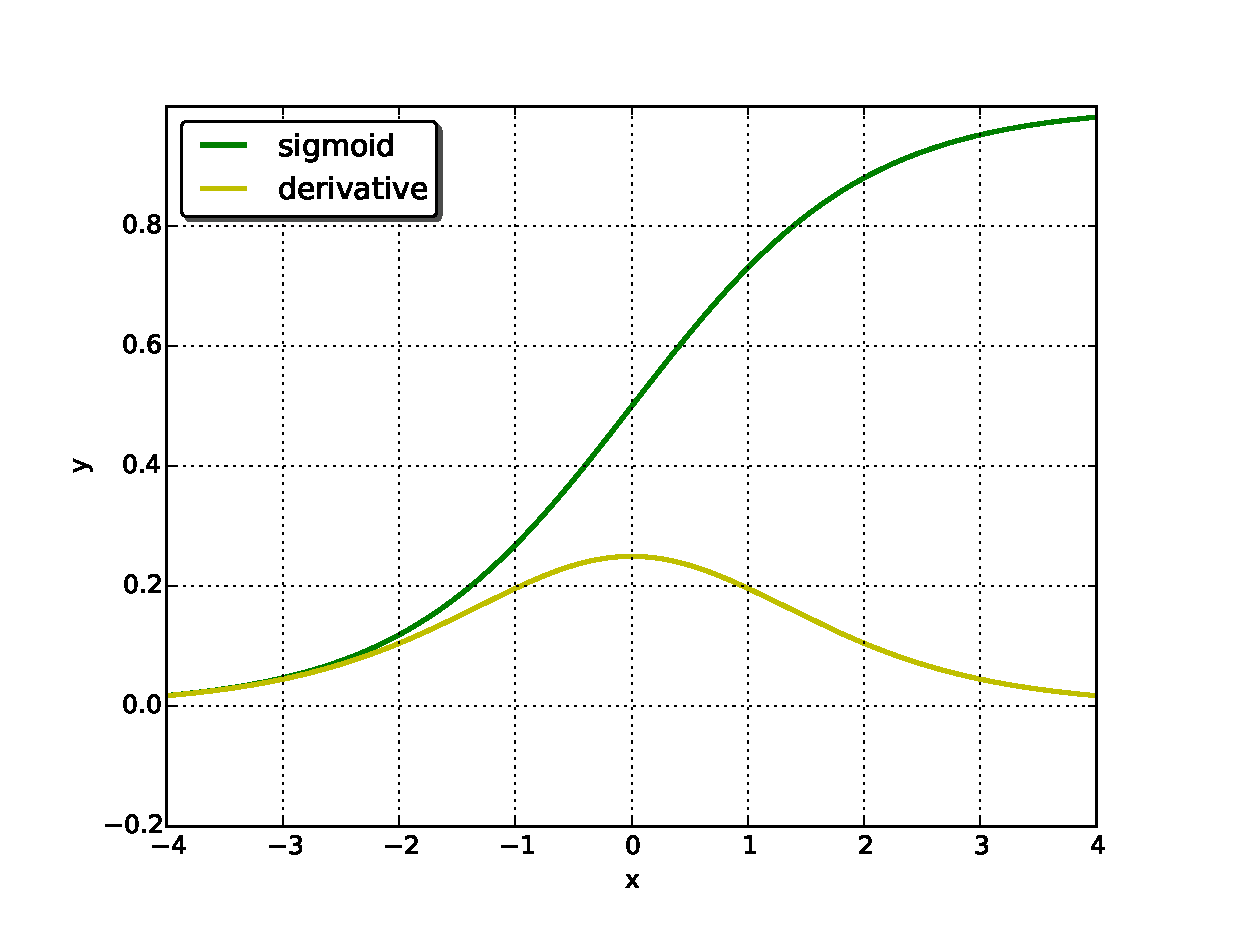
\includegraphics[width=0.9\textwidth]{sigmoid_and_deriv.eps}
  \caption{sigmoid and it's derivative}
\label{sigmoid_plot}
\end{figure}

\paragraph{Tanh}

As we can see from figure \ref{tanh_plot} tanh (and it's derivative) have a behaviour similar to the sigmoid one; Again we have two saturation region towards
infinity: that's typical of all squashing functions.

\begin{align}
 tanh(x)&=\frac{e^x-e^{-x}}{e^x+e^{-x}} \\
 tanh'(x)&= 1 - tanh^2(x)  
\end{align}

\begin{figure}[h]
  \centering
    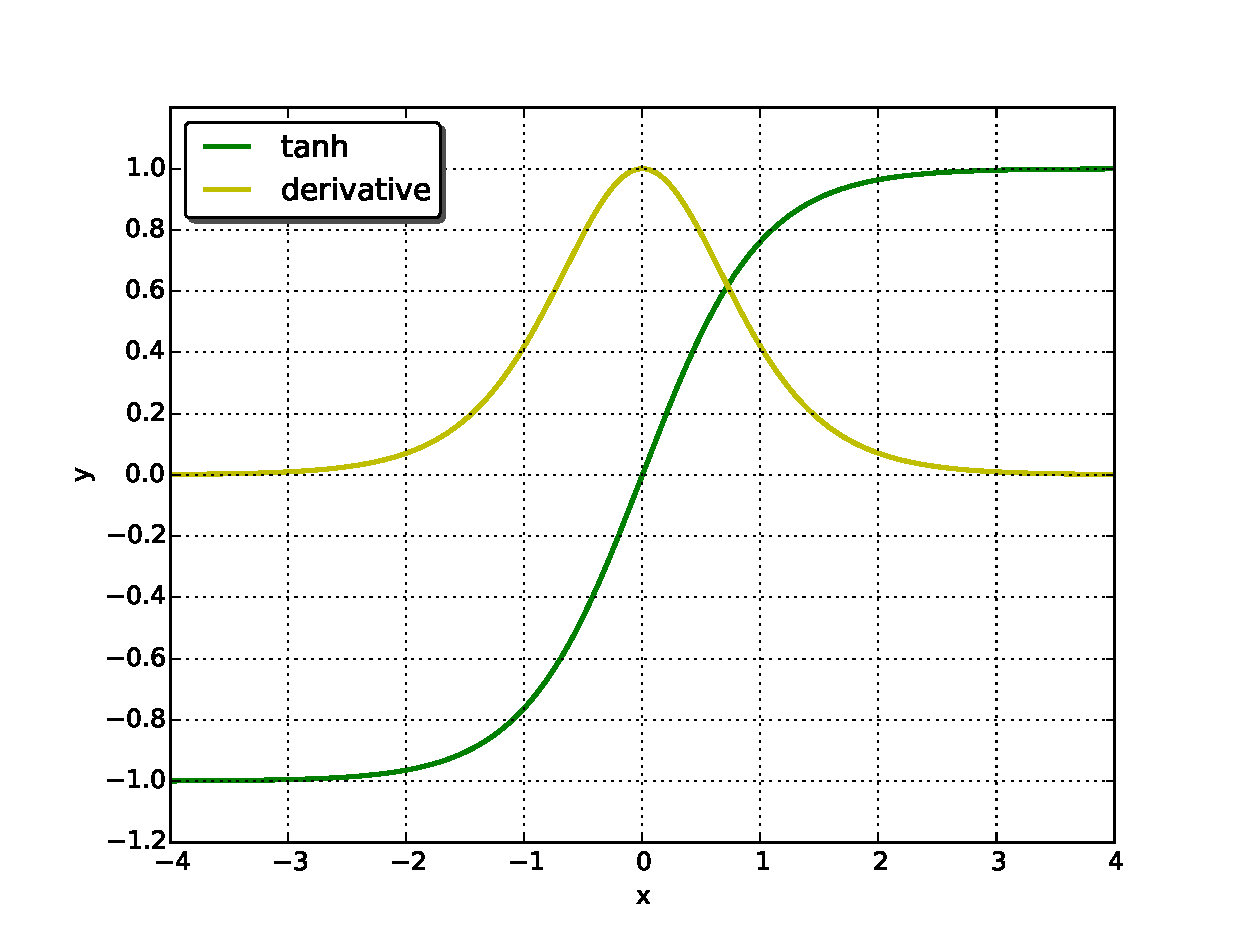
\includegraphics[width=0.9\textwidth]{tanh_and_deriv.eps}
  \caption{tanh and it's derivative}
\label{tanh_plot}
\end{figure}

\paragraph{ReLU}


\begin{align}
  ReLU(x)&=\begin{cases}
    x & \text{if $x>0$}.\\
    0 & \text{otherwise}.
  \end{cases} \\ 
   ReLU'(x)&=\begin{cases}
    1 & \text{if $x>0$}.\\
    0 & \text{otherwise}.
  \end{cases}
\end{align}


ReLU is a bit different from other activation function seen so far: the main difference is that's it's not a squashing function.
As we can see from figure \ref{relu_plot}, ReLU's derivative is the step function; it has only one \textit{saturation} region $(-\inf, 0]$ and a region in which is always takes value one, $(0,+\inf]$
This leads to the fact that we cannot learn to 'turn on' a switched off neuron ($x<0$), but we have no \textit{saturation} region toward $+\inf$.

\begin{figure}[h]
  \centering
    \includegraphics[width=0.9\textwidth]{relu_and_deriv.eps}
  \caption{ReLU and it's derivative}
\label{relu_plot}
\end{figure}

  \section{On expressiveness}
  In this section we will investigate the expressive power of neural networks, presenting some results that motivate the use of neural networks as learning
models and underline the differences between the two paradigm of FNNs and RNNs. 

One of the first import results regarding the expressive power of neural networks it's due to Hornik et al. \cite{Hornik89} which basically states
\textit{``Multilayered feed foward networks with at least one hidden layer, using an arbitrary squashing function, can approximate virtually any function
of interest to any desired degree of accuracy provided sufficiently many hidden units are available''}.

To give a more formal result we need first to define what \textit{approximate to any degree of accuracy means}, this concept is captured in definition
\ref{dens_compact}
 
\begin{defn}
 A subset S of $\mathbb{C}^n$ (continuoos functions in $\mathbb{R}^n$) is said to be \textit{uniformly dense on compacta in} $\mathbb{C}^n$ if $\forall$
 compact set $K\subset \mathbb{R}^n$ holds: $\forall \epsilon >0$, $\forall g(\cdot) \in \mathbb{C}^n$ $\exists f(\cdot) \in S$ such that 
 $\underset{x \in K}{\text{sup  }} \norm{f(x)-g(x)}<\epsilon$ 
 \label{dens_compact}
\end{defn}

Hornik result is contained in theorem \ref{universal_approx}.
\begin{thm}
 For every squashing function $\sigma$, $\forall n\in \mathbb{N}$, feed forward neural
 networks with one hidden layer are a class of functions which is \textit{uniformly dense on compacta in} $\mathbb{C}^n$
\label{universal_approx}.
\end{thm}

Theorem \ref{universal_approx} extends also to Borel measurable functions, please see \cite{Hornik89} for more details.

A survey of other approaches, some of which constructive, which achieve similar results can be found in \cite{Scarselli98}
At the moment I don't know of any results concerning ReLU activation function.

This results implies that FNN are \textit{universal approximators}, this is a strong argument for using such models in machine learning.
It's important to notice, however, that the theorem holds if we have \textit{sufficiently many} units. In practice the number of units will bounded
by the machine capabilities and by computational time, of course greater the number of units greater will be the learning time. This will limit
the expressiveness of the network to a subset of all measurable functions. 

BOUNDS?
\\\\Let's now turn our attention to RNNs and see how the architectural changes, namely the addition of backward links, affect the expressive power of the model.
It suffice to say that RNNs are as powerfull as turing machine. Siegelman and Sontag \cite{Siegelmann91turingcomputability} proved the existence 
of a finite neural network, with sigmoid activation function, which simulates a universal Turing machine. Hy{\"o}tyniemi \cite{Hyotyniemi96turingmachines} proved, equivalently,
that turing machine are recurrent neural network showing how to build a network, using instead ReLU activation function, that performs step by step 
all the instruction of a computer program.
Hy{\"o}tyniemi work is particularly interesting because it shows how to construct a network that simulate an algorithm written a simple language equivalent to a turing machine.
For each instruction type (increment,decrement,conditional branch,...) a particular setting of weights and neuron is devised allowing the net so simulate step by step the behaviour of the program. 
In the program equivalent network there are a unit for each program variable and one or two, depending on the instruction type, units for each program instruction.
This is very interesting from an expressiveness point of view since it bounds the number of units we ought to use with the length of the algorithm we are trying to reproduce.

For better understanding the implications of this fact, imagine how many complex function you can express with short algorithms, for example fractals (approximations).
It's worth underling the difference with feed forward neural networks where a large number of units seems to be required. This seems to suggest that FFNNs and RNNs differ mainly in a manner of 
representation, where FNNs use space to define a somehow explicit mapping from input to output, RNNs use time to implicitly define an algorithm responsible for such mapping. 

This seems extremely good news, since we could simulate turing machines, hence all algorithms we can think of, using a recurrent neural network with a relatively small number of units; 
recall that for FFNN we had to suppose infinitely many units to obtain the universal approximator property.
Of course there is a pitfall: we can simulate any turing machine but we have to allow sufficiently many time steps and choose a termination criterion.
This is of course impractical, and we don't use RNNs in this way. Usually the number of time steps is choose to be equal to the input sequence length. This of course restrict the class of algorithm
we can learn with RNNs. A particular class of algorithms suited to be learned by such models is that of algorithms consisting in one loop, inside which some invariants are enforced. The output, step by step,
depends on cycle invariants.






\chapter{An historical review of proposed solutions}
  distinction between architectural and non architectural solutions, historical review 

  
\subsection{Long short-term memory} 

\textit{Long short-term memory} (LSTM) were proposed (1997) by Hochreiter and Schmidhuber\cite{lstm} as a novel network 
structure to address the vanishing gradient problem, which was first studied by Hochreiter (1991) in his diploma 
thesis, a milestone of deep learning.

The idea behind this structure is to enforce a constant error flow, that is to say, to have constant gradient norm, 
thus preventing the gradient to vanish. This is done by introducing special types of neurons called \textit{memory 
cells} and \textit{gate units}. As we can see by looking at figure \ref{lstm_neuron}, a memory cell is essentially a 
neuron with a self connection with unitary weight, whose input and output are managed by two multiplicative neurons: 
the gate units.


\tikzstyle{nn_style}=[->,shorten >=1pt,auto,node distance=1.5cm,
  thick,
  neuron/.style={circle,fill=white!50,node distance=1cm,draw,minimum size=0.7cm,font=\sffamily\normalsize},
  missing/.style={circle,font=\sffamily\Large,node distance=0.95cm},
  label/.style={node distance=1.2cm,rectangle,fill=white!50,draw=none,minimum size=0.7cm,font=\sffamily\normalsize},
  layer/.style={rectangle,fill=white!50,draw,minimum width=0.8cm,font=\sffamily\Large},
  loopStyle/.style={in=120,out=60, distance=2.5cm},
  weight/.style = {above,sloped,pos=0.3},]
\begin{figure}[h]
  \centering
  \begin{tikzpicture}[nn_style]

    %horizontal line
    \node[neuron]	(c1)       					{$\times$};
    \node[layer] 	(s_mem)	[right of=c1,	node distance=1.5cm] 	{$\Sigma$};
    \node[neuron]	(mem)	[right of=s_mem,node distance=1.5cm]	{$m_j$};
    \node[layer] 	(h)	[right of=mem,	node distance=1.5cm] 	{$h$};
    \node[neuron]	(c2)	[right of =h,	node distance=1.5cm]	{$\times$};
    \node[label]  	(out)	[right of=c2,	node distance=2.2cm]	{$\phi_j$};
    
    \path[->] (c1) 	edge []   (s_mem)
	      (s_mem) 	edge []   (mem)
	      (mem) 	edge []   (h)
	      (h) 	edge []   (c2)
	      (c2) 	edge []   (out);
	     
    
    %loop	     
    \path[->] (mem) edge [loop, in=90,out=120, distance=0.8cm, anchor=south ] node [align=center, pos=0.7] 
 {$1$} (s_mem);

    
    %above inputs
    \node[layer] 	(g)	[above of=c1,	node distance=1.5cm] 	{$g$};
    \node[layer] 	(s_in)	[above of=g,	node distance=1.2cm] 	{$\Sigma$};
    \node[missing]	(i2)	[above of=s_in, node distance=1.2cm]	{$\hdots$};
    \node[neuron]	(i3)	[right of=i2, 	node distance=1cm]	{};
    \node[neuron]	(i1)	[left of=i2, 	node distance=1cm]	{};

    
    \path[->] (s_in) 	edge [anchor=west]	node[]{}	(g)
	      (g) 	edge [anchor=west]   	node[]{$a_j$}	(c1)
	      (i1)	edge []   					(s_in) 
      	      (i3)	edge []   					(s_in);
      	      
      	      
    %below gate input unit
    \node[layer] 	(sig_in)	[below of=c1,		node distance=1.5cm] 	{$\sigma$};
    \node[layer] 	(s_gate_in)	[below of=sig_in,	node distance=1cm] 	{$\Sigma$};
    \node[missing]	(gi2)		[below of=s_gate_in, 	node distance=1.2cm]	{$\hdots$};
    \node[neuron]	(gi3)		[right of=gi2, 		node distance=1cm]	{};
    \node[neuron]	(gi1)		[left of=gi2, 		node distance=1cm]	{};

    
    \path[->] (s_gate_in) 	edge [anchor=west]	node[]{}	(sig_in)
	      (sig_in) 		edge [anchor=west]	node[]{$u_j$} 	(c1)
	      (gi1)		edge []   (s_gate_in) 
      	      (gi3)		edge []   (s_gate_in);
      	      
      	      
    %below gate output unit
    \node[layer] 	(sig_out)	[below of=c2,		node distance=1.5cm] 	{$\sigma$};
    \node[layer] 	(s_gate_out)	[below of=sig_out,	node distance=1cm] 	{$\Sigma$};
    \node[missing]	(go2)		[below of=s_gate_out, 	node distance=1.2cm]	{$\hdots$};
    \node[neuron]	(go3)		[right of=go2, 		node distance=1cm]	{};
    \node[neuron]	(go1)		[left of=go2, 		node distance=1cm]	{};

    
    \path[->] (s_gate_out) 	edge [anchor=west]	node[]{}	   (sig_out)
	      (sig_out) 	edge [anchor=west]	node[]{$o_j$}   (c2)
	      (go1)		edge []						   (s_gate_out) 
      	      (go3)		edge []						   (s_gate_out);

    %enclosing rectangle
    \node[rectangle,dashed,fill=none,draw,minimum height=3.2cm,minimum width=8.1cm] at (3.4, 0.5) (memoryCell)	{};
    \node[label]  (memoryLabel)	at(3.5,2.1)	{Memory cell};


      	      
\end{tikzpicture}
\caption{Memory cell and gate units of LSTM network}
\label{lstm_neuron}
\end{figure}

The memory cell and the gate units behave accordingly to the following:

\begin{equation}
 u_j^t = \sigma[\mat{W_u}\cdot\vec{x_t} + \mat{U}_u\cdot\vec{\phi}_{t-1}]_j
\end{equation}

\begin{equation}
 o_j^t = \sigma[\mat{W_o}\cdot\vec{x_t} + \mat{U}_o\cdot\vec{\phi}_{t-1}]_j
\end{equation}

\begin{equation}
a^t_j\defeq g[\mat{W}\cdot\vec{x_t} + \mat{U}\cdot\phi_i^t]_j
\end{equation}
\begin{equation}
 m_j^t\defeq a_j\cdot u_j^t + (1 \cdot m_j^{t-1})
\label{mem_update}
\end{equation}
\begin{equation}
 \phi_j\defeq h(m_j^t)\cdot o^t_j
\end{equation}


% \begin{equation}
% u^t_j\defeq \sigma(\sum_i w_{ui}\cdot u^{t-1}_j)
% \end{equation}
% \begin{equation}
% o^t_j\defeq \sigma(\sum_i w_{oi}\cdot o^{t-1}_j)
% \end{equation}
% 
% 
% \begin{equation}
% a^t_j\defeq g(\sum_i w_{ij}\cdot \phi_i^t)
% \end{equation}
% \begin{equation}
%  m_j^t\defeq a_j\cdot u_j^t + (1 \cdot m_j^{t-1})
% \label{mem_update}
% \end{equation}
% \begin{equation}
%  \phi_j\defeq h(m_j^t)\cdot o^t_j
% \end{equation}

As we can see from equation \ref{mem_update}, the value of the memory cell $m(t)$ remains constant as long as the input 
gate $u$ doesn't ``open'' causing a ``write'' operation. Similarly the output $o$ of the memory cell, which is 
connected with 
the other neurons of the network, is controlled by an output gate: the memory will have a non zero output only if the 
output gate opens, which we could call a  a ``read'' operation. As for constant error flow it is ensured because the 
memory cell has only a self-loop with unitary weight.

Memory cells, guarded by gate units can be employed in networks with different topology alongside traditionally 
input, output and hidden units. Another way to look at this kind of architecture is to think of memory cells as units 
able to store one bit of information, even for long periods of time, hence able to learn distant time correlations 
between inputs.

As we have seen these network units are specifically designed to store information, through the use of gates; these 
gates however are no different from other units, apart from the fact they are multiplicative units, hence without 
further precautions, the networks would incur in the same vanishing problem it aimed to resolve. In fact LSTM comes with 
a proper learning algorithm: essentially errors arriving at memory cells inputs are not propagated back in time, only 
the error within the memory cell gets propagated; in other words gradients are truncated taking into account only the 
self-connection of the memory cells and not it's other input connections, hence providing constant error flow.

LSTM units have proven to be very successful in various tasks and even at present times (2015), they continue to be 
employed. In recent implementations however, alongside small modifications, as the introduction of other gates, LSTM 
architecture is often used without the original learning algorithm which is often replaced by a standard stochastic 
gradient descend as done in \cite{lstmGraves}.









% \chapter{Some results}
%   \section{Vanishing gradient solutions}
%   In section \ref{vanishing_sec} were established some weak bounds on the weight matrix $\mat{W}^{rec}$ whose crossing entails the arising of
the vanishing gradient problem.

It would be nice to find some lower bounds on the weight matrix which don't allow an exponential decay of long term components. However since activation
functions can all have zero value, we cannot establish any lower bound different from zero.

However what we are really interested in is the cost of the paths which cross \textit{active} neurons because, structurally, \textit{switched off} neurons don't
contribute to the gradient. Formally we define


\begin{defn}{Active neuron}
A neuron $j$ is said to be active if $$\sigma(a_j)>\tau$$
 
\end{defn}






To overcame this problem we return to the previously introduced graph formulation where we consider each component 
$\frac{\partial \vec{a}_i^t}{\partial \vec{a}_j^k}$ as the sum path cost.



\begin{equation} 
\frac{\partial \vec{a}_i^t}{\partial \vec{a}_j^k} = \sum_{q\in P(j)} \sum_{l \in P(q)} \hdots \sum_{h : i \in P(h)} w_{qj} \hdots w_{jh} \cdot \sigma'(a_j^k)\sigma'(a_q^{k+1}) \hdots \sigma'(a_i^{t-1})
\label{expanded_mem}
\end{equation}

\appendix
\chapter{Notation}

Let $F:\mathbb{R}^N \rightarrow \mathbb{R}^M$ be defined by
\begin{equation}
F(\vec{x}) = (f_1(\vec{x}),f_2(\vec{x}),\cdots,f_M(\vec{x}))) \text{    for some  } f_i:\mathbb{R}^N \rightarrow \mathbb{R}
\end{equation}

\begin{defn}[Derivative with respect to a vector]
 We define the derivative of $F(x(\vec{w}))$ with respect to a vector $\vec{w}$ of $p$ elements as the $M \times p$ matrix
\begin{equation}
\frac{\partial F}{\partial \vec{w}} \triangleq
\begin{bmatrix}
   \frac{\partial f_1}{\partial \vec{w}_1}    & \frac{\partial f_1}{\partial \vec{w}_2}                & \cdots      & \cdots       & \frac{\partial f_1}{\partial \vec{w}_p}  \\
   \frac{\partial f_2}{\partial \vec{w}_1}    & \frac{\partial f_2}{\partial \vec{w}_2}                & \cdots      & \cdots       & \frac{\partial f_2}{\partial \vec{w}_p}  \\
   \vdots                & \vdots           & \vdots      & \vdots       &\vdots\\
   \frac{\partial f_M}{\partial \vec{w}_1}    & \frac{\partial f_M}{\partial \vec{w}_2}                & \cdots      & \cdots       & \frac{\partial f_M}{\partial \vec{w}_p}
\end{bmatrix}
\end{equation}
\end{defn}


\begin{defn}[Derivative with respect to a matrix]
We define the derivative of $F(\vec{x}(\mat{W}))$ with respect to a matrix $\mat{W}$, being $W_j$ the $j^{th}$ column of a 
$p\times m$ matrix $W$ as the $M\times (p \cdot m )$ matrix:
\begin{equation}
\frac{\partial F}{\partial \mat{W}} \triangleq
\left[
\begin{array}{c|c|c|c}
\frac{\partial F}{W_1} & \frac{\partial F}{W_2} & \cdots & \frac{\partial F}{W_m} \\
\end{array}
\right]
\end{equation}
\end{defn}
Please note that according to this definitions $\nabla f(x)$ with $f:\mathbb{R}^N \rightarrow \mathbb{R}$ corresponds to $\frac{\partial f}{\partial\vec{x}}^T$.

\begin{defn}[Immediate derivative]
Consider a recurrence 
$$a^k(\vec{x}) =F(\vec{x}(\vec{w})) +  R(a^{k-1}(\vec{x}(\vec{w})), \dots, a^0(\vec{x}(\vec{w})))$$
We define the immediate derivative of $a^k(\vec{x}(\vec{w})))$ with respect to the vector $\vec{w}$
the matrix 
\begin{equation}
	\frac{\partial^+ a^k}{\partial \vec{w}} \defeq \frac{\partial F}{\partial \vec{w}}.
\end{equation}
\end{defn}





\newpage
% \nocite{*}		 % Mostra in bibliografia anche gli oggetti non citati 
\bibliography{biblio}{}
\bibliographystyle{plain}


\end{document}     